\section{Обзор существующих исследований}
	Циклоны используются для удаления твёрдых частиц из газовых потоков с конца 19 века. Простая конструкция, низкие затраты на производство и обслуживание и адаптивность к широкому диапазону рабочих параметров сделали циклоны одними из наиболее часто используемых промышленных фильтров. 
	
		Эффективность циклонов определяется степенью очистки воздуха $\eta$, равной отношению количества частиц данного диаметра, задержанных циклоном к полному числу частиц. В силу того, что принцип работы этих фильтров основан на инерциальных силах, они имеют низкую эффективность для частиц, диаметром менее $5 \mu m$.
	
	Существует огромное количество конфигураций, однако противоточные циклоны с тангенциальным входом \textit{(рисунок \ref{fig:cycloneOverview})} чаще всего используются для очистки воздуха в промышленности. Такая конфигурация описывается девятью безразмерными параметрами \textit{(таблица \ref{tableCyclone})}, отнесёнными к масштабу длины $D$, характеризующему диаметр фильтра \cite{DirgoLeith}.\\
  \begin{minipage}{0.6\textwidth}
    \captionof{table}{Геометрия фильтра}
			\begin{tabular}{l l}
				\hline
				\label{tableCyclone}
				Диаметр цилиндра, & $D$\\
				Диаметр выходной трубы, & $D_e$\\
				Высота входного канала, & $a$\\
				Ширина входного канала, & $b$\\
				Длина выходной трубы, & $h_e$\\
				Полная высота фильтра, & $H$\\
				Высота цилиндра, & $h$\\
				Диаметр нижнего сечения фильтра, & $B$\\
				Высота пылесборника, & $h_d$\\
				Диаметр пылесборника, & $D_d$\\
			\end{tabular}
    \end{minipage}
    \hspace{1em}
  \begin{minipage}{0.35\textwidth}
    \label{fig:cycloneOverview}
    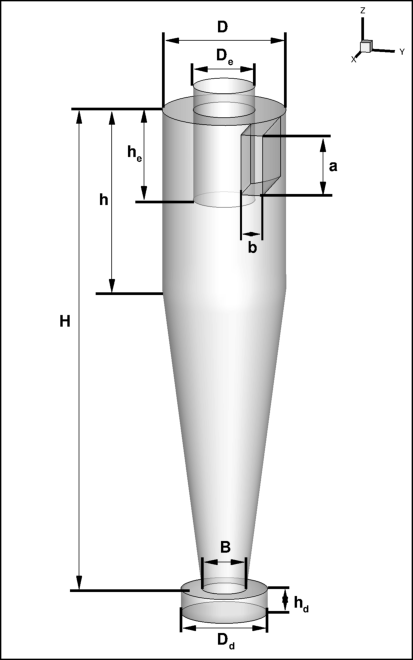
\includegraphics[scale=0.375]{Geometry}
				\captionof{figure}{Схема фильтра}
  \end{minipage}
	\subsection{Теоретические исследования}
		\hspace{1em}
		Среди теоретических исследований течения в циклонах особо выделим статью Dirgo, Leith \cite{DirgoLeith}. Авторы статьи систематизировали различные модели, выделив три основных подхода к описанию фильтра.
			\subsubsection{Критический диаметр: время полёта частиц}
			\subsubsection{Критический диаметр: статика}
			\subsubsection{Эффективность}
	\subsection{Экспериментальные исследования}
		\hspace{1em}Существует большое количество работ по экспериментальному исследованию течения с искривлёнными линиями тока. Среди них стоит выделить достаточно подробный эксперимент, приведённый в статье Monson et al. \cite{Monson}. Авторы статьи проводят численное и экспериментальное исследование турбулентного течения воздуха в U-образном канале.
		
		Экспериментальному моделированию циклонов также уделено немало внимания. Среди статей, приводящих экспериментальные данные по турбулентному течению в циклонах, можно, опять же, отметить детальное исследование течения в циклоне модели Stairmand, описанное в статье J. Dirgo, D. Leith \cite{DirgoLeith}. В этой статье приведены данные для профилей скорости в нескольких сечениях фильтра для большого диапазона рабочих параметров. К сожалению, авторы используют модифицированную модель фильтра, в которой масштаб $D = 0.375m$ отличается от классического $D = 0.205m$, предложенного в работе Stairmand \cite{Stairmand}, поэтому экспериментальные данные неприменимы к моей работе, в которой рассматривается именно классическая модель фильтра.
	\subsection{Численные исследования}
		\hspace{2em}Численному моделированию течения в циклонах посвящено очень много инженерных исследований.
	%Численные исследования
\newpage
%Обзор существующих моделей
